%!TEX root = ../physical-olympics-2.tex
\chapter{刚体}


\section{刚体的物理描述}
近代以前人们意识到了物质世界的\emph{连续性}(continuum),\,同时针锋相对地也提出了\emph{原子论}(atomism).\,原子最简单的模型就是质点,\,而调和物质连续性与原子学说的中间模型就是\emph{刚体}(rigid body)模型.\,刚体是不允许形变发生的系统.\,由牛顿力学对质点的讨论推广到质点系的讨论,\,使我们也很容易将相关结论进一步推广到刚体.

由于刚体上一点受力,\,则整体同时运动起来,\,这个模型与相对论力学体系是不兼容的.\,具体来说,\,相互作用必须以有限的速度传播,\,否则就违背了因果律.\,刚体不符合因果律这一时空的固有结构.\,在很多相对论情境下将招致矛盾的结果.

刚体的物理学量是哪一些呢?\,必要的内禀的属性是其质量的分布.\,某一默认时刻$t_0$刚体占据了空间区域$\Omega_0$,\,由大量体积微元$\ud V$(记做$\ud^3\bs{R}_0$)组成,\,则刚体的总质量为:
\[m=\int\limits_{\Omega_0}\rho(\bs{R}_0)\ud^3\bs{R}_0=\int\limits_{\Omega_0}\ud m\]

\begin{wrapfigure}[17]{o}[-10pt]{7cm}
\vspace{-0.4cm}
\centering
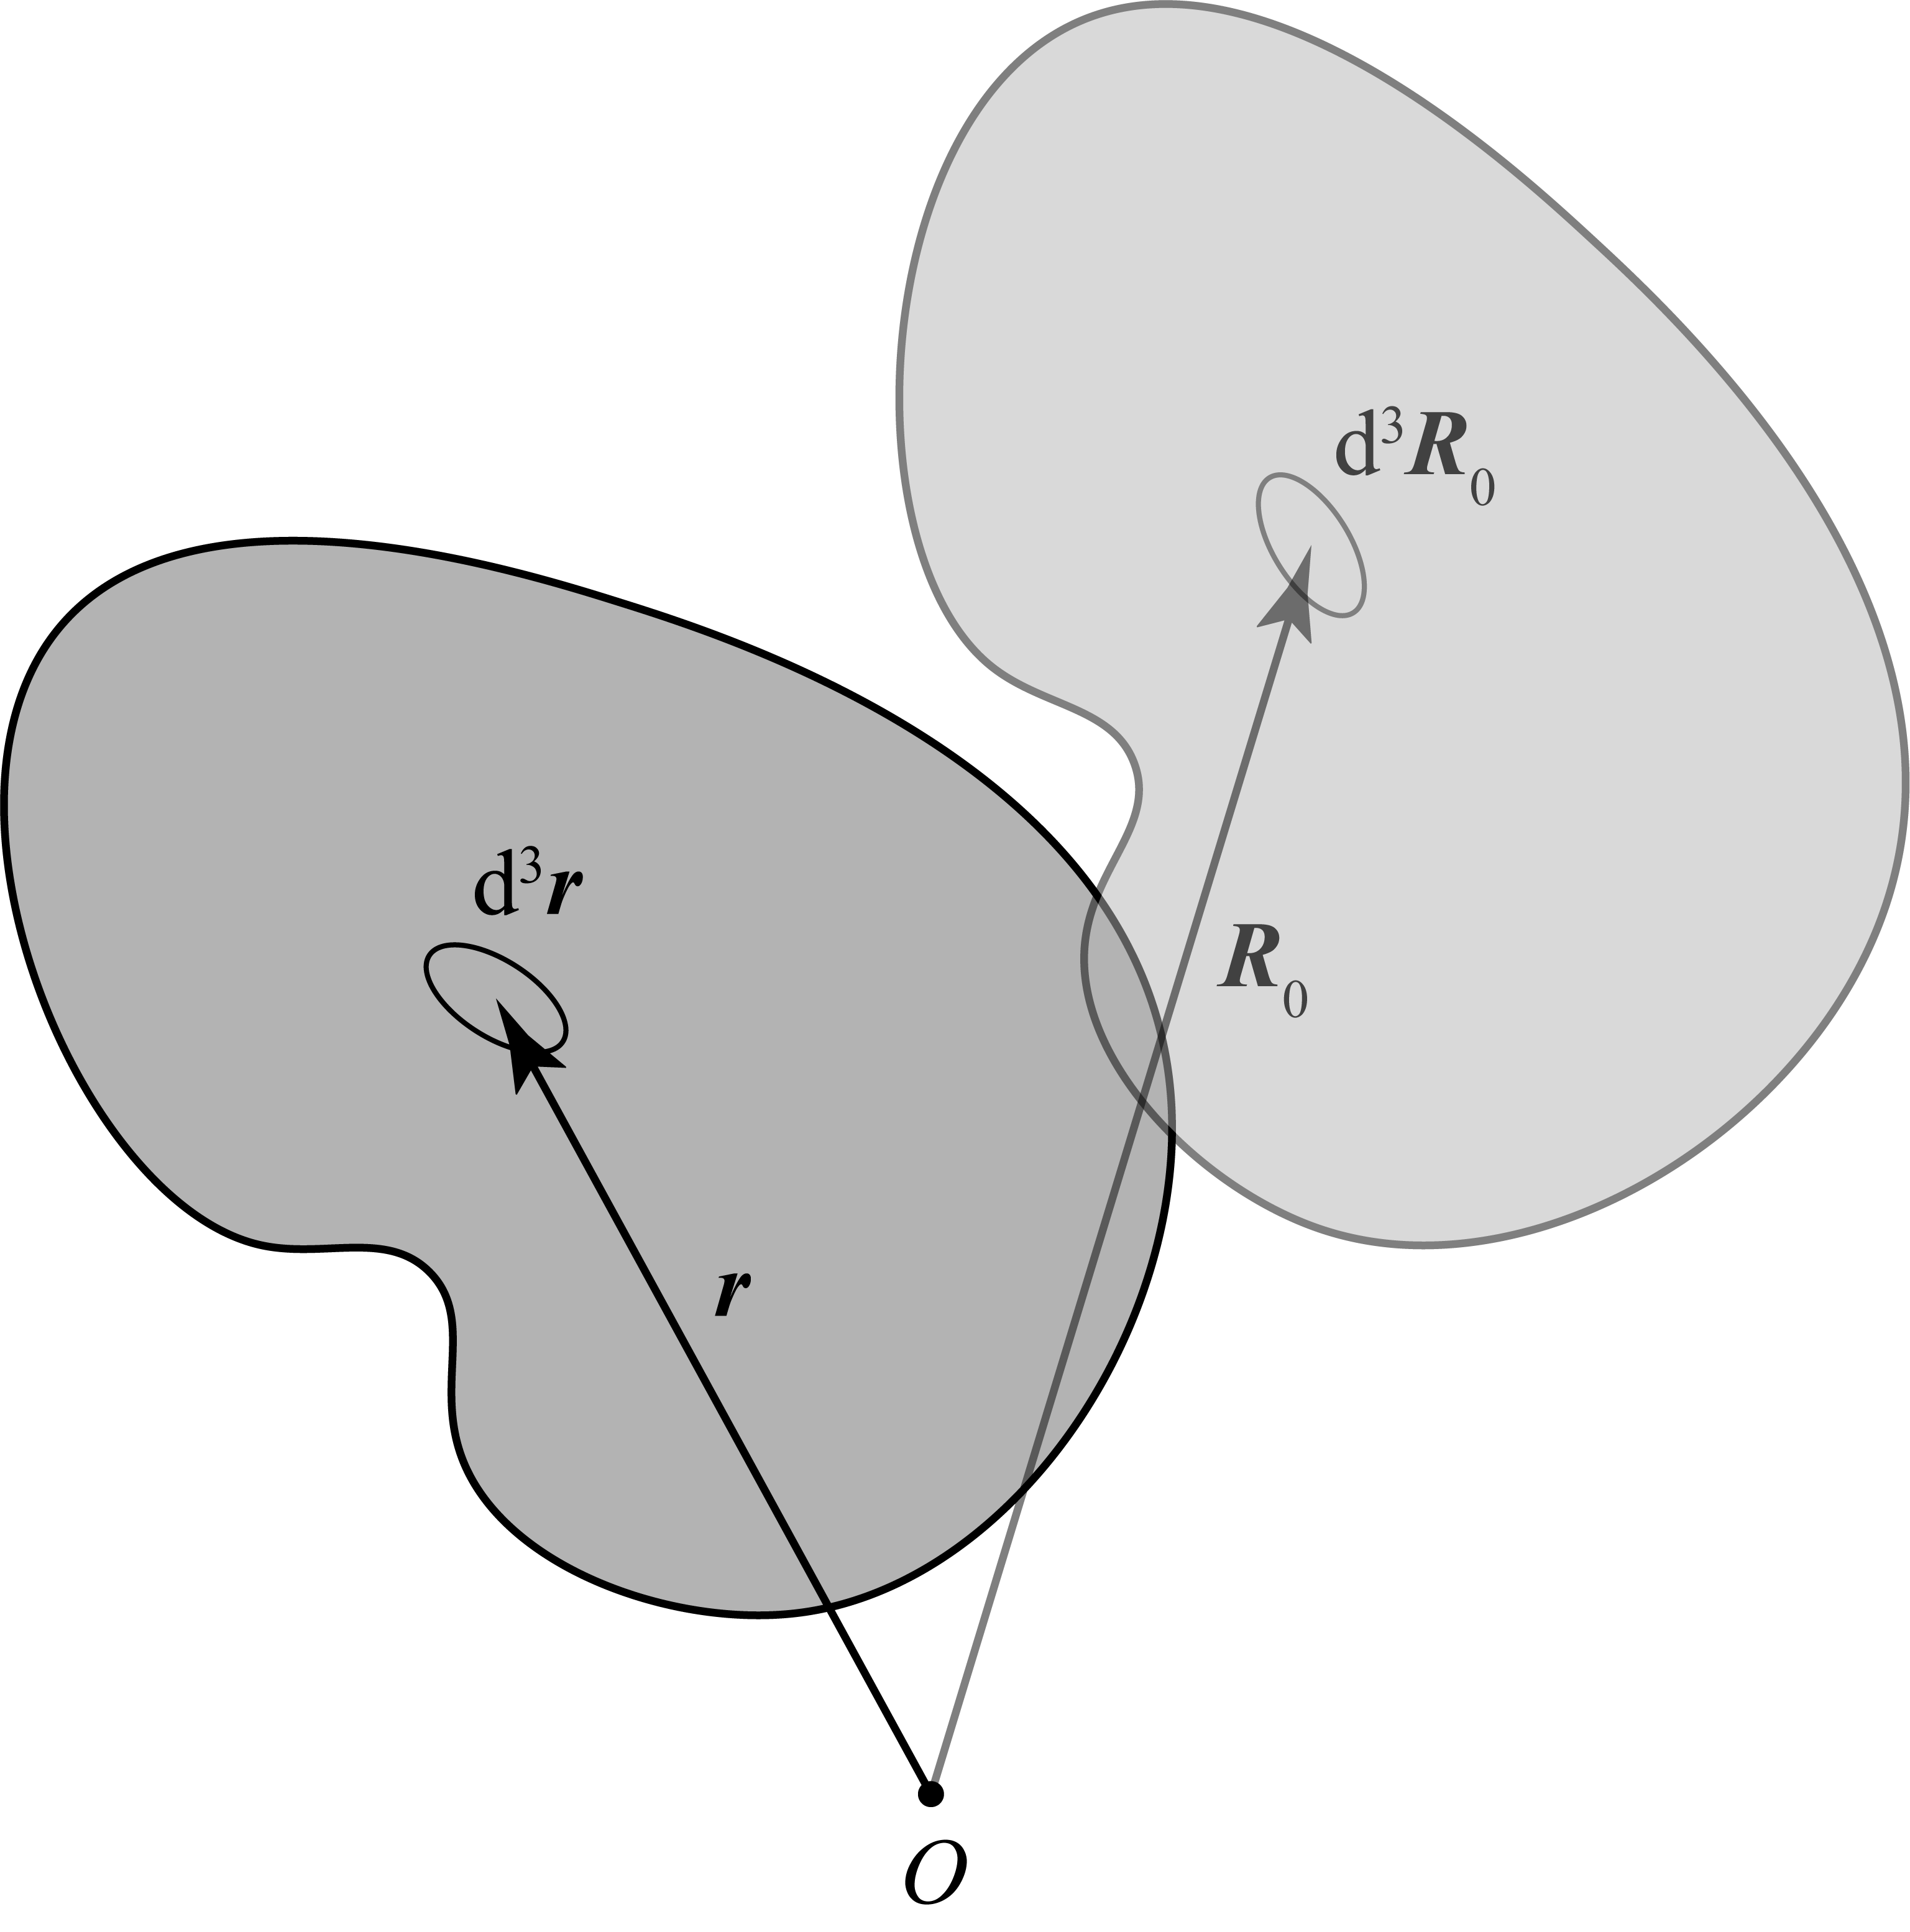
\includegraphics[width=7cm]{image/6-6-1.png}
\caption{刚体的描述}
\end{wrapfigure}
随着刚体的运动,\,原来在$\bs{R}_0$处的体积元现在在$t$时刻位于$\bs{r}$处,\,整个刚体的运动由一个多元映射来定义:
\[f:\quad \bs{R}_0,\,t\;\;\longrightarrow\;\; \bs{r}(\bs{R}_0,\,t)\]

刚体的刚性的要求,\,使得这个映射必须保持体积元的不变性:
\[f:\quad \ud^3\bs{R}_0\in\Omega_0\;\;\longrightarrow\;\; \ud^3\bs{r}\in\Omega \quad ;\quad \ud^3\bs{R}_0=\ud^3\bs{r}=\ud V\]

而且所有这个体积元内的所有内禀属性,\,这里包括密度都不能变.\,所以质量元$\ud m$也是不变的.\,从而刚体具有不变的总质量.\,马上就会发现,\,\emph{质量几何}(mass geometry)对刚体的动力学来说也十分重要.\,质量几何研究质量对特定原点$O$的各级\emph{矩}(moment).\,其中零级矩即为质量:
\[\phantom{}^0M=m=\int\limits_\Omega \ud m\]

一级矩是个矢量,\,它定义了刚体的\emph{质心}(center of mass)的位置:
\[\phantom{}^1M_i=mr_{Ci}=\int\limits_\Omega r_i\ud m\]
\[\bs{r}_C=\frac{\int\limits_\Omega \bs{r}\ud m}{\int\limits_\Omega \ud m}\]

二级矩则是一个张量,\,它的九个分量代表\emph{惯量积}(product of inertia):
\[\phantom{}^2M_{ij}=\int\limits_\Omega r_ir_j\ud m\]

这些矩和原点的选取有关,\,随着刚体的运动也会不断变化,\,这三阶矩的信息对刚体动力学来说就是充分的了,\,通过后面的动力学可以发现,\,刚体的运动完全依赖于外力和这三阶矩.\,如果要研究广义相对论里的引力波辐射问题,\,更高阶的矩才变得重要起来.

刚体的运动可以被我们更精确地描述,\,在$t_0$时刻建立固定在刚体上,\,沿$x,y,z$三方向的单位矢量$\bs{e}_1,\bs{e}_2,\bs{e}_3$,\,那么刚体的运动同时也把三个矢量旋转到新的三个方向:
\[f:\quad \bs{e}_i\;\longrightarrow\; \bs{\varepsilon}_i\]

这三个矢量仍然要互相垂直,\,且长度为一.\,这在数学上导致了可以通过这三个矢量的导数定义\emph{角速度}(angular velocity)矢量的结果:
\[\dot{\bs{\varepsilon}}_i=\bs{\omega}\times\bs{\varepsilon}_i\]

\begin{wrapfigure}[15]{o}[-10pt]{7cm}
\vspace{-0.7cm}
\centering
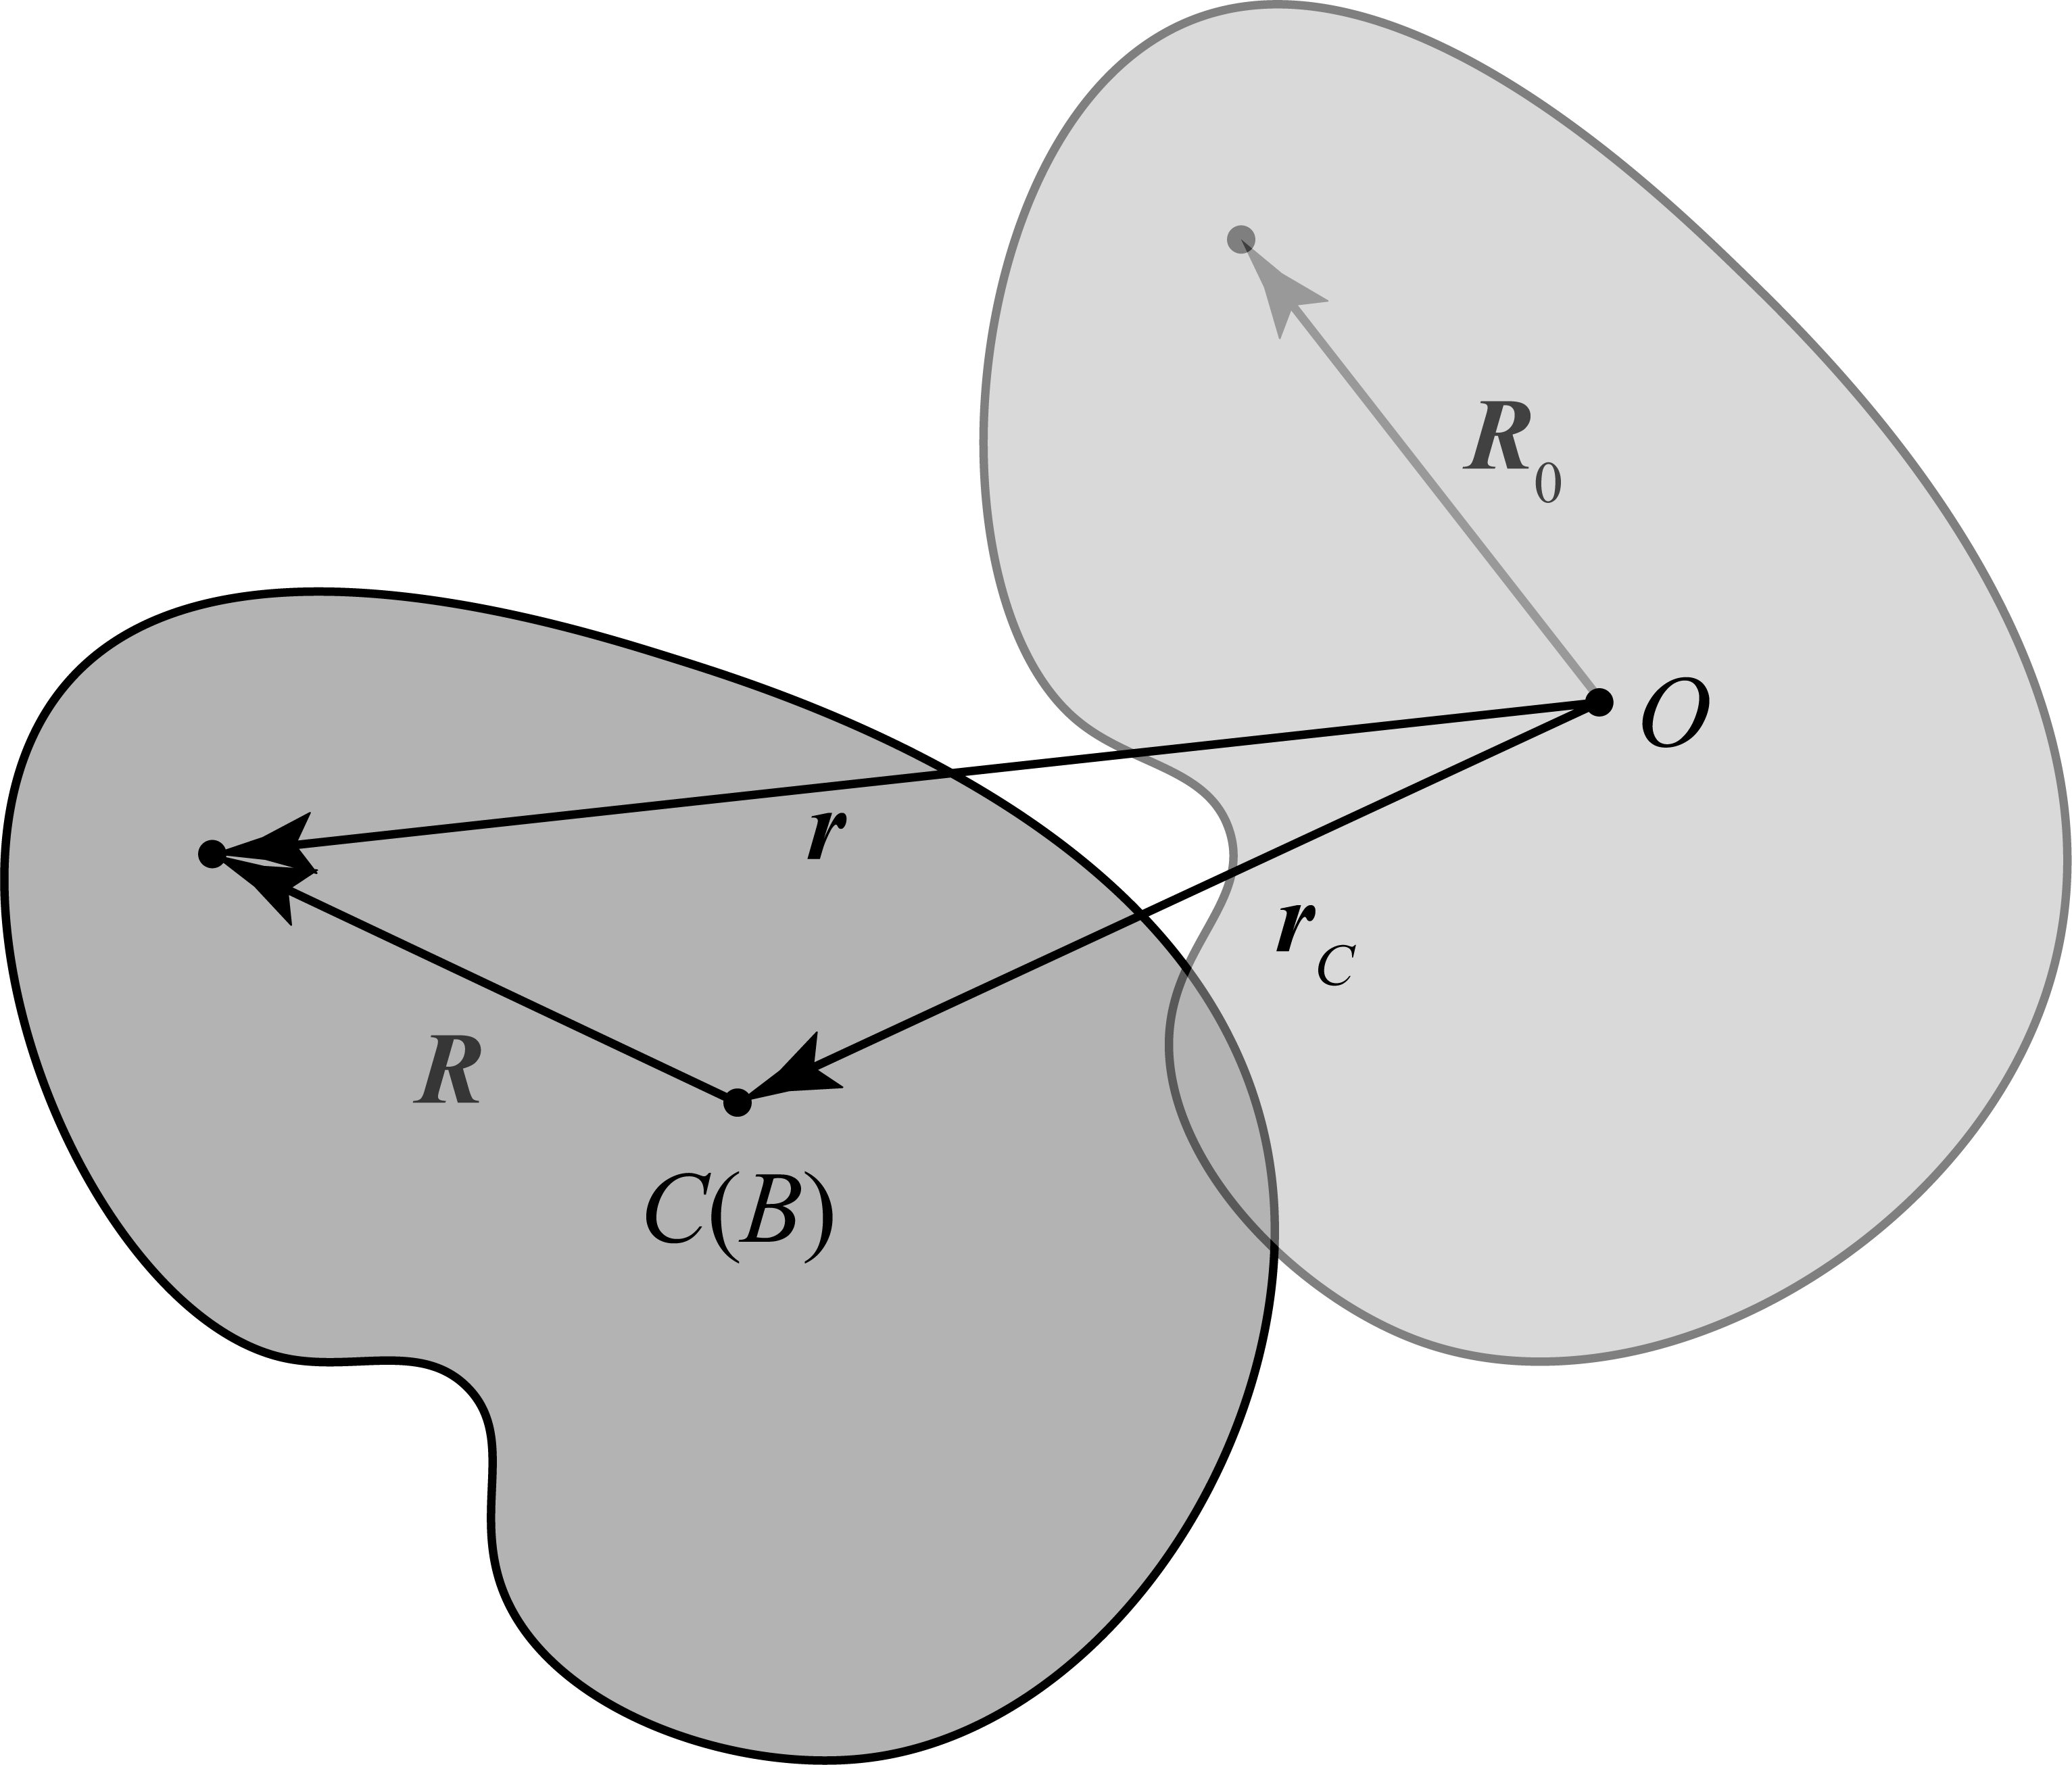
\includegraphics[width=7cm]{image/6-6-2.png}
\caption{基点法}
\end{wrapfigure}
十分类似于旋转参考系的变换的运动学,\,刚体的运动实际上就是有一个唯一的旋转参考系固连在刚体上,\,以后称作\emph{刚体系}(reference system of rigid body),\,要研究的刚体上各个点速度实际上就是刚体系中定点的运动.\,于是习惯上我们采用\emph{基点法}(method of base point)来计算刚体上任意点的运动学量.\,定义\emph{基点}(base point)为$t_0$时刻$\bs{R}_0=\bs{0}$的点$B$,\,之后的位矢为$\bs{r}_B$,\,对应的基点速度加速度为$\bs{v}_B,\,\bs{a}_B$,\,而刚提上待研究的点相对基点的位矢为$\bs{r}-\bs{r}_B=\bs{R}$,\,那么该点的速度加速度即为:
\[\bs{v}=\bs{v}_B+\bs{\omega}\times\bs{R}\]
\[\bs{a}=\bs{a}_B+\bs{\omega}\times(\bs{\omega}\times\bs{R})+\dot{\bs{\omega}}\times\bs{R}\]

出于动力学的考虑,\,基点$B$一般就取做质心$C$.\,作用在刚体上$\bs{r}$处的力$\bs{F}$固然对原点会有力矩$\bs{M}$,\,但是为了研究使刚体自身转动的效应,\,考虑到这个力同时也会使得质心运动起来,\,故我们重视这个力相对质心的力矩$\bs{M}_C$:
\[\bs{M}=\bs{r}\times\bs{F}\]
\[\bs{M}_C=\bs{R}\times\bs{F}\]

刚体受到一个力系${\bs{F}_i}$的作用,\,那么以下六个定理则来自于之前的动力学理论:
\[\sum_i\bs{F}_i=\frac{\ud \bs{p}}{\ud t}\quad ; \quad \sum_i\bs{F}_i=m\bs{a}_C\]
\[\sum_i \bs{v}_i\cdot \bs{F}_i=\frac{\ud }{\ud t}(\frac{1}{2}m\bs{v}_C^2+E_{kr})\quad ;\quad \sum_i(\bs{v}_i-\bs{v}_C)\cdot \bs{F}_i=\frac{\ud E_{kr}}{\ud t}\]
\[\sum_i \bs{r}_i\times \bs{F}_i=\frac{\ud }{\ud t}(\bs{r}_C\times m\bs{v}_C+\bs{L}_r)\quad ;\quad \sum_i \bs{R}_i\times \bs{F}_i=\frac{\ud \bs{L}_r}{\ud t}\]

前两个式子实际上几乎没有区别,\,因为刚体的总动量其实就是质心动量$\bs{p}=m\bs{v}_C$.\,后面几个式子则涉及到相对(平动)质心系的能量与角动量.\,它们与质量二级矩有着密切的联系,\,我们在第三讲\ref{6.3}阐明.\,现在我们写出相对质心系能量角动量的定义:
\[E_{kr}=\int\limits_\Omega \frac{1}{2}(\bs{\omega}\times \bs{R})^2\ud m\]
\[\bs{L}_r=\int\limits_\Omega \bs{R}\times(\bs{\omega}\times \bs{R})\ud m\]




\section{平面平行运动}
一个底面磨平的物体贴在平坦的地面上运动给人以\emph{平面平行运动}(plane-parallel motion)的概念.\,其他的一些物体运动特征也相似于它:\,黑板刷在黑板上的运动,\,车轮在直行时的滚动...\,它们的特征是:\,刚体任何一个体积元都在一个特定的平面上运动,\,而这些平面又彼此平行.\,对于这样的运动基点法只需要给出质心$C$的位矢$\bs{r}_C$和对$t_0$时刻刚体转过的角度$\theta$即可.\,自由度就只有3个.\,角速度与角加速度即可用角度的导数来给出$\omega=\dot{\theta},\,\beta=\ddot{\theta}$.\,一般来说,\,在垂直于这些平面方向要么由于动力学对称性不需要也不存在任何作用力.\,要么这些力作为约束平面对物体的约束力而不在我们考虑范围内.\,所以我们对一些物理对象做如下修改:\,
\begin{itemize}
\item 所有参考点改成垂直平面过该点的参考轴.\,并约定其正方向为垂直纸面向外.\,这样的轴方向为$z$方向,\,而运动平面的方向为$x-y$平面.
\item 与之对应地,\,刚体绕轴的转动,\,产生的角速度方向以逆时针为正.\,这样角速度方向与约定的正方向一致.\,以后在处理的时候,\,往往被作为标量而处理.
\item 关于\emph{转动惯量}(rotational inertia):\,现在就可以把质元到转动轴---不妨把它设为$x=y=0$的轴---的距离用来计算其二级矩,\,对应的概念就叫做对这根轴的转动惯量:
\[I=\int \rho^2\ud m=\int (x^2+y^2)\ud m=M_{xx}+M_{yy}\]

正如上式所示,\,它是9个惯量积中的特定2个的和.
\item 轴的三种可能性:\,一是空间中的定轴,\,一是刚体上的固连轴,\,还有可能是在空间中或是相对刚体都不静止的动轴.\,后面就会发现,\,定轴用角动量定律;\,固连轴几乎都取过质心的轴,\,有转动定律;\,而动轴也有瞬时转动轴的特例,\,可以证明有瞬时转动轴定律存在.\,无论哪种情况,\,转动惯量如上一点定义.\,这样在定轴和瞬时转动轴情况下,\,它有可能变成一个随时间变化的值$I(t)$
\item 动能的计算:\,动能的定义不需要做任何修正.\,而且概念本身也并不依赖与轴的选取.\,只是,\,其计算方法变得简单,\,而且有两种算法:
\begin{itemize}
	\item 如果是瞬时转动轴,\,那么动能直接是:
	\[T(t)=\frac{1}{2}I(t)\omega^2(t)\]

	\item 如果是定轴或过质心的轴,\,事实上任何对定轴$O$计算刚体动能最终都必须由柯尼希定律转化为两项:\,一项是质心$C$的\emph{轨道运动}(orbital motion)动能,\,和相对质心的\emph{自旋运动}(spin motion)带来的动能.\,这也是唯一正确的分解方式:\,质心$C$换成其它相对刚体固定的点都是错的.\,而刚体相对质心的转动惯量就不会是变化的了,\,记作$I_C$.\,从而两个动能可以表示为:
	\[T_C=\frac{1}{2}mv_C^2(t)\quad,\quad T_S=\frac{1}{2}I_C\omega^2(t)\quad,\quad T=T_C+T_S\]
\end{itemize}

\item 角动量的计算:\,角动量的定义就需要做修正了.\,我们仅仅选取角动量的$z$分量,\,这是因为要么刚体是薄的,\,对平面上的点角动量本来就只有$z$分量,\,要么刚体虽然有$x-y$平面上的角动量但其动力学效果是产生一些约束它在$x-y$平面上运动的我们不感兴趣的约束力.\,所以角动量也和角速度一样可以被视作标量,\,对任何点$P$的角动量$J$可以被定义为\footnote{注意即使$P$在动,\,$\bs{v}$也没有必要改为$\bs{v}-\bs{v}_P$.\,}:
\[J_P=\bs{e}_z\cdot \int \bs{\rho}_P\times \bs{v}\ud m\]

式中,\,$\bs{\rho}_P$是从$P$轴垂直地指向每一个质元$\ud m$的矢径.\,根据$P$点不同的选取方法,\,有以下几种计算方法:
\begin{itemize}
	\item 如果是瞬时转动轴,\,这种情况我们只在较少情况下使用.\,那么对它的角动量直接是:
	\[J(t)=I(t)\omega(t)\]

	\item 如果是定轴,\,刚体角动量也必须由柯尼希定律转化为两项:\,一项是质心$C$的\emph{轨道角动量}(orbital angular momentum)$L$,\,和相对质心的\emph{自旋角动量}(spin angular momentum)$S$.\,这也是唯一正确的分解方式:\,质心$C$换成其它相对刚体固定的点都是错的.\,刚体对质心的转动惯量$I_C$是常数.\,从而两者可以表示为:
	\[L=\bs{e}_z\cdot [m\bs{r}_C(t)\times \bs{v}_C(t)]\quad,\quad S=I_C\omega(t)\quad,\quad J=L+S\]
	
	\item 其它动轴.\,除非变换参考系,\,否则一般极少被考虑.
\end{itemize}
\end{itemize}

平面平行运动的刚体的自由度为3,\,所以只需要3个方程就足以求解其运动,\,这三个方程通常取做质心运动定律和绕质心的\emph{转动定律}(rotation law):
\[\sum_i F_{xi}=m a_{Cx}\]
\[\sum_i F_{xi}=m a_{Cx}\]
\[\sum_i M_{i}=I_{C} \beta\]

\section{空间刚体运动*}\label{6.3}

我们来定义空间刚体的转动惯量,\,首当其冲的一点是,\,沿不同方向的轴的转动惯量是不一样的.\,那么我们改变一下定义.\,把转动惯量视作从角速度到角动量的一个映射,\,为了简洁,\,把映射直接写成一个点乘,\,后面就知道其合理性:
\[\bs{I}:\quad \bs{\omega}\to \bs{L}=\bs{I}\cdot\bs{\omega}\]

那么这个映射一定是线性的.\,这是因为如果角速度为$\bs{\omega}=\lambda_1\bs{\omega}_1+\lambda_2\bs{\omega}_2$.\,那么根据第一节给出的角动量计算方法:
\[\bs{L}=\int \bs{r}\times(\bs{\omega}\times \bs{r})\ud m\]

得到$\bs{I}\cdot\bs{\omega}=\lambda_1 \bs{L}_1+\lambda_2 \bs{L}_2$

那么它就一定可以写作一个矩阵:

\[\bs{I}=\begin{bmatrix}I_{x}&I_{xy}&I_{xz}\\I_{yx}&I_{y}&I_{yz}\\I_{zx}&I_{zy}&I_{z}\end{bmatrix}\]

背后具有这样的原理:\,如果我们让角速度为$(1,\,0,\,0)$,\,把此时角动量计算出来写作$(I_x,\,I_{xy},\,I_{xz})$.\,同理如果角速度为$(0,\,1,\,0)$时的角动量为$I_{yx},\,I_{y},\,I_{yz}$,\,角速度为$(0,\,0,\,1)$时的角动量为$I_{zx},\,I_{zy},\,I_{z}$.\,那么任意角速度情况都可以视作以上三种情况的线性叠加:
\[(\omega_x,\,\omega_y,\,\omega_z)=\omega_x(1,\,0,\,0)+\omega_y(0,\,1,\,0)+\omega_z(0,\,0,\,1)\]

所以相应的角动量也是直接叠加的:
\[\bs{L}=\bs{I}\cdot\bs{\omega}\quad :\quad \left\{\begin{array}{ccc}L_x &=& I_{x}\omega_x+I_{xy}\omega_y+I_{xz}\omega_z\\L_y &=& I_{yx}\omega_x+I_{y}\omega_y+I_{yz}\omega_z\\L_z &=& I_{zx}\omega_x+I_{zy}\omega_y+I_{z}\omega_z\end{array}\right.\]

那么把上式写成一个矩阵的形式是再合适不过的了:
\[\begin{bmatrix}L_{x}\\L_{y}\\L_{z}\end{bmatrix}=\begin{bmatrix}I_{x}&I_{xy}&I_{xz}\\I_{yx}&I_{y}&I_{yz}\\I_{zx}&I_{zy}&I_{z}\end{bmatrix}\begin{bmatrix}\omega_{x}\\\omega_{y}\\\omega_{z}\end{bmatrix}\]

所以是不是说在这个意义下刚体的转动惯量$\bs{I}$就是一个矩阵?\,这依然有不妥的地方.\,因为如果换一个坐标系,\,这个矩阵就会变化,\,但是从角速度到角动量的映射是不会发生变化的.\,我们有一种更严谨的定义方法,\,是把转动惯量形式上写成如下的\emph{张量}(tensor)形式:
\[\bs{I}=I_x\bs{e}_x\bs{e}_x+I_y\bs{e}_y\bs{e}_y+I_z\bs{e}_z\bs{e}_z+I_{xy}\bs{e}_x\bs{e}_y+I_{xz}\bs{e}_x\bs{e}_z+I_{yx}\bs{e}_y\bs{e}_x+I_{yz}\bs{e}_y\bs{e}_z+I_{zx}\bs{e}_z\bs{e}_x=I_{zy}\bs{e}_z\bs{e}_y\]

其中$\bs{e}_i\bs{e}_j$是一种新定义的\emph{并矢}(dyadic)运算的结果,\,这种运算把两个矢量自由地并在一起,\,满足按照分量的分配律,\,但是不满足交换律,\,即形成的并矢,\,即一个张量的九个基,\,对称的两个基是不被认为相等的:
\[\bs{e}_i\bs{e}_j\neq \bs{e}_j\bs{e}_i\]

张量因为代表了物理量之间的映射而具有了物理意义.\,但是如果觉得这一层意义不够明显,\,我们可以把张量代表的映射表示出来,\,这一步是通过张量与矢量的点乘操作体现出来的.\,事实上我们定义这个点乘一样地符合分配律,\,而基之间的点乘符合:
\[(\bs{e}_i\bs{e}_j)\cdot \bs{e}_k=\bs{e}_i(\bs{e}_j\cdot \bs{e}_k)\]

即如果$j=k$则就是$\bs{e}_i$,\,如果不等于,\,那就是零.\,这就不难验证,\,的确能把之前的矩阵式,\,按照张量的方式理解为:
\[\bs{L}=\bs{I}\cdot\bs{\omega}\]

最后,\,如果把之前的角动量定义式按照三重矢积公式,\,按分量展开可以得到:
\[\bs{L}=\int \bs{r}\times(\bs{\omega}\times \bs{r})\ud m=\int \left(\sum_i r_i^2 \sum_j \omega_j \bs{e}_j-\sum_i r_i \bs{e}_i\sum_j r_j\omega_j \right)\ud m\]

利用之前定义的二级矩:
\[\bs{L}=(M_{xx}+M_{yy}+M_{zz})\sum_i \omega_i \bs{e}_i-\sum_{ij}M_{ij}\omega_j\bs{e}_i\]

写成分量形式为:
\[\left\{\begin{array}{ccc}L_x &=&(M_{yy}+M_{zz})\omega_x+M_{xy}\omega_y+M_{xz}\omega_z\\L_y &=& M_{yx}\omega_x+(M_{xx}+M_{zz})\omega_y+M_{yz}\omega_z\\L_z &=& M_{zx}\omega_x+M_{zy}\omega_y+(M_{xx}+M_{yy})\omega_z\end{array}\right.\]

对比之前的惯量张量,\,我们发现了实际上惯量张量的非对角线分量其实就是对应的惯量积,\,从而还具有对称性:
\[I_{ij}=I_{ji}=M_{ij}\]

而对角线分量却不是惯量积.\,它是真正对这些轴的转动惯量,\,如$x$轴:
\[I_x=M_{yy}+M_{zz}\]

数学上可以证明,\,对任何点,\,存在特殊的三条正交轴$x-y-z$,\,称为\emph{主轴}(principal axes),\,可以使得惯量积都为零,\,只剩下三个主转动惯量:

\[\begin{bmatrix}L_{x}\\L_{y}\\L_{z}\end{bmatrix}=\begin{bmatrix}I_{x}&0&0\\0&I_{y}&0\\0&0&I_{z}\end{bmatrix}\begin{bmatrix}\omega_{x}\\\omega_{y}\\\omega_{z}\end{bmatrix}\]

即:
\[\bs{L}=(I_x\omega_x,\,I_y\omega_y,\,I_z\omega_z)\]

